\chapter{Casos de Uso}\label{apendice.A}
\section{Introducción}
\subsection{Propósito}
El propósito de este documento es describir de una forma clara y concreta cada uno de los casos de uso definidos para el sistema web a implementar.
\subsection{Alcance}
Los casos de uso presentados en este documento representan los requerimientos que se desean implementar en el sistema web para el aprendizaje colaborativo.
\subsection{Definiciones, acrónimos y abreviaciones}
\begin{enumerate}
  \item CU: Caso de uso
  \item SAC: Sistema para el aprendizaje colaborativo
\end{enumerate}
\clearpage
\section{Catálogo de actores}
En la  \autoref{fig:actores} se puede ver los actores que participan en el Sistema Jigsaw Coding y en la \autoref{tab:actores} se encuentra una breve descripción de cada uno de ellos.
\begin{figure}
  \centering
  % Requires \usepackage{graphicx}
  \fbox{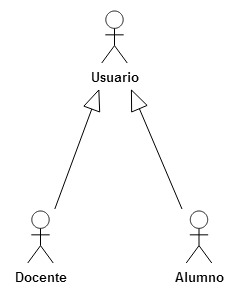
\includegraphics[scale=0.6]{figuras/casosdeuso/actores.jpg}}\\
  \caption[Diagrama de actores]{Diagrama de actores}
  \label{fig:actores}
\end{figure}

\begin{longtable}{L{3cm}L{7cm}}
\caption{Actores}
\label{tab:actores}\\
    \toprule[0.8mm]
    ACTOR & DESCRIPCIÓN \\
    \midrule[0.6mm]
    Usuario & Persona que usará el sistema web de tiempo real para el aprendizaje colaborativo.\\
    \midrule
    Docente & Es la persona responsable de crear y dirigir las sesiones de clase que serán aplicadas a los alumnos. Además, el docente es el responsable de las evaluaciones que rendirán los alumnos una vez terminada cada sesión de clase.\\
    \midrule
    Alumno & Es la persona que será instruida en temas de algoritmos y programación a través de cada sesión diseñada por el docente.\\
    \bottomrule[0.8mm]
\end{longtable}
\clearpage
\begin{landscape}
\section{Diagramas de casos de uso}
\subsection{Casos de uso}
\begin{figure}[!h]
  \centering
  % Requires \usepackage{graphicx}
  \fbox{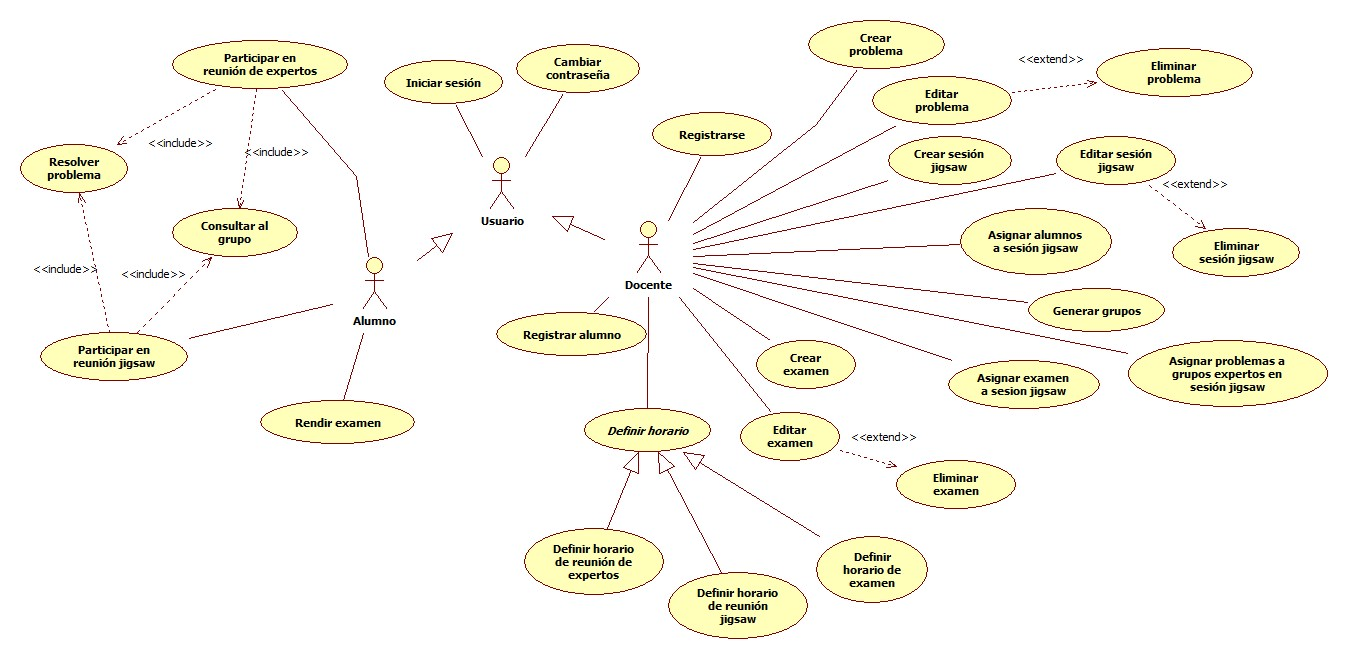
\includegraphics[scale=0.4]{figuras/casosdeuso/casos_de_uso.jpg}}\\
  \caption[Casos de uso]{Diagrama de casos de uso para el sistema JigsawCoding}
  \label{fig:casos_de_uso}
\end{figure}
\end{landscape}
\clearpage

\section{Especificaciones de Casos de Uso}

\subsection{Iniciar sesión}
\begin{longtable}{|c|L{10cm}|}
	\toprule[0.8mm]
	Código &  CUS-\casodeuso\\  \midrule
	Nombre &  INICIAR SESIÓN.\\  \midrule
	Descripción & El caso de uso describe los pasos para acceder al Sistema Jigsaw Coding.\\  \midrule
	Actores & Docente, Alumno. \\  \midrule
	Precondiciones &  Ninguna.\\  \midrule
	Postcondiciones &  Ninguna.\\  \midrule
	Flujo básico &  \begin{enumerate}
		\item El docente o alumno escribe su correo electrónico como usuario.
		\item El docente o alumno escribe su Password.
		\item El docente o alumno presiona el botón Ingresar.
	\end{enumerate}
	\\  \midrule
	Flujo alternativo &  Ninguno.\\  \bottomrule[0.8mm]
\end{longtable}
\clearpage
\subsection{Registrar Alumno}
\begin{longtable}{|c|L{10cm}|}
  \toprule[0.8mm]
  % after \\: \midrule or \cline{col1-col2} \cline{col3-col4} ...
  Código &  CUS-\casodeuso\\  \midrule
  Nombre &  REGISTRAR ALUMNO.\\  \midrule
  Descripción & El caso de uso inicia cuando el docente selecciona la opción registrar nuevo alumno. Luego completa la información del alumno y el caso de uso termina cuando se presiona la opción Guardar. \\  \midrule
  Actores & Docente. \\  \midrule
  Precondiciones &  El docente debe estar logueado en el sistema.\\  \midrule
  Postcondiciones &  Ninguna.\\  \midrule
  Flujo básico &  \begin{enumerate}
                    \item El docente selecciona la opción para registrar un nuevo alumno.
                    \item El sistema muestra el formulario para completar los datos del alumno.
                    \item El docente completa los campos DNI, Apellido Paterno, Apellido Materno, Nombres, Email, Sexo, Email, Contraseña, Repetir Contraseña.
                    \item El sistema valida el formato del DNI, apellidos, nombres, email.
                    \item El sistema valida que el email no esté registrado en el sistema.
                    \item El sistema verifica que los campos contraseña y repetir contraseña sean idénticos.
                    \item El sistema registra al nuevo alumno en el sistema.
                  \end{enumerate}
  \\  \midrule
  Flujo alternativo &  Ninguno.\\  \bottomrule[0.8mm]
\end{longtable}
\clearpage
\subsection{Crear Problema}

%\begin{tabular}{|c|L{9cm}|}
%  \midrule
%  % after \\: \midrule or \cline{col1-col2} \cline{col3-col4} ...
%  Código &  CUS-\casodeuso\\  \midrule
%  Nombre &  \\  \midrule
%  Descripción &  \\  \midrule
%  Actores &  \\  \midrule
%  Precondiciones &  \\  \midrule
%  Postcondiciones &  \\  \midrule
%  Flujo básico &  \\  \midrule
%  Flujo alternativo &  \\  \midrule
%\end{tabular}

\begin{longtable}{|c|L{9cm}|}
  \toprule[0.8mm]
  % after \\: \midrule or \cline{col1-col2} \cline{col3-col4} ...
  Código & CUS-\casodeuso \\  \midrule
  Nombre & CREAR PROBLEMA. \\  \midrule
  Descripción & El caso de uso inicia cuando el usuario accede al sistema y elige la opción crear problema. Luego el usuario redacta el enunciado y demás observaciones sobre el problema y finaliza el caso de uso. \\  \midrule
  Actores & Docente. \\  \midrule
  Precondiciones & El usuario de ser un Docente y estar logueado en el sistema. \\  \midrule
  Postcondiciones & El docente verá en la lista de problemas el problema recién creado. \\  \midrule
  Flujo básico & \begin{enumerate}
                   \item El docente elige la opción NUEVO PROBLEMA.
                   \item El sistema solicita al docente ingresar el título y enunciado del problema.
                   \item El docente escribe el título y enunciado del problema.
                   \item El docente selecciona la opción GUARDAR.
                   \item El sistema guarda el nuevo problema.
                 \end{enumerate}    \\  \midrule
  Flujo alternativo & Ninguno. \\  \bottomrule[0.8mm]
\end{longtable}
\clearpage
\subsection{Crear sesión jigsaw}
\begin{longtable}{|c|L{10cm}|}
  \toprule[0.8mm]
  % after \\: \midrule or \cline{col1-col2} \cline{col3-col4} ...
  Código &  CUS-\casodeuso\\  \midrule
  Nombre &  CREAR SESIÓN JIGSAW.\\  \midrule
  Descripción &  El caso de uso inicia cuando el usuario accede al sistema y elige la opción de crear una nueva sesión de clase jigsaw; luego ingresa los datos necesarios de la sesión de clase y el caso de uso termina cuando la nueva sesión es creada satisfactoriamente en el sistema.\\  \midrule
  Actores &  Docente.\\  \midrule
  Precondiciones & El usuario debe ser un Docente y estar logueado en el sistema. Los grupos expertos deben haber sido creados. \\  \midrule
  Postcondiciones & El docente verá en el listado de clases la nueva sesión creada. \\  \midrule
  Flujo básico & \begin{enumerate}
                    \item El docente abre un formulario para crear una nueva sesión de clase jigsaw.
                    \item El docente rellena el campo tema.                    
                    \item El docente indica el número total de grupos expertos a incluir en la sesión.
                    \item El docente selecciona la opción Guardar.
                    \item El sistema graba la información de la nueva sesión jigsaw.
                 \end{enumerate}
   \\  \midrule
  Flujo alternativo & Ninguno. \\  \bottomrule[0.8mm]
\end{longtable}
\clearpage
\subsection{Modificar sesión jigsaw}
\begin{longtable}{|c|L{10cm}|}
  \toprule[0.8mm]
  % after \\: \midrule or \cline{col1-col2} \cline{col3-col4} ...
  Código &  CUS-\casodeuso\\  \midrule
  Nombre &  MODIFICAR SESIÓN JIGSAW\\  \midrule
  Descripción & El caso de uso inicia cuando el usuario accede al sistema y selecciona la opción modificar sesión jigsaw. El usuario realiza los cambios que requiera y luego finaliza el caso de uso. \\  \midrule
  Actores &  Docente.\\  \midrule
  Precondiciones &  El usuario debe ser un Docente y debe estar logueado en el sistema. Debe existir una sesión jigsaw en el sistema.\\  \midrule
  Postcondiciones &  Ninguna.\\  \midrule
  Flujo básico & \begin{enumerate}
                    \item El docente selecciona una sesión jigsaw creada y luego elige la opción editar.
                    \item El docente puede cambiar el total de grupos expertos y el tema o examen de la sesión jigsaw.
                    \item El docente selecciona la opción FINALIZAR.
                    \item El sistema guarda los cambios realizados a la sesión jigsaw.

                 \end{enumerate}
   \\  \bottomrule[0.8mm]
  Flujo alternativo &  Ninguno.\\  \midrule
\end{longtable}
\clearpage
\subsection{Asignar alumnos a sesión jigsaw}
\begin{longtable}{|c|L{10cm}|}
	\toprule[0.8mm]
	% after \\: \midrule or \cline{col1-col2} \cline{col3-col4} ...
	Código &  CUS-\casodeuso\\  \midrule
	Nombre &  ASIGNAR ALUMNOS A SESIÓN JIGSAW\\  \midrule
	Descripción &  El caso de uso inicia cuando el docente selecciona la opción Asignar Alumnos para un determinada sesión jigsaw, luego agrega a los alumnos y cuando presiona la opción guardar, el caso de uso termina.\\  \midrule
	Actores &  Docente.\\  \midrule
	Precondiciones &  El usuario de ser un Docente y estar logueado en el sistema. Deben existir alumnos registrados.\\  \midrule
	Postcondiciones &  Ninguna.\\  \midrule
	Flujo básico &    \begin{enumerate}
		\item El docente selecciona la opción Asignar Alumnos en la lista de sesiones jigsaw.
		\item El docente arrastra a los alumnos desde la lista de disponibles hacia la lista de alumnos para la sesión jigsaw.
		\item El docente presiona la opción Guardar.
		\item El sistema guarda la lista de participantes de la sesión jigsaw.
	\end{enumerate}  \\ \midrule
	Flujo alternativo & Ninguno. \\  \bottomrule[0.8mm]
\end{longtable}
\clearpage
\subsection{Generar grupos}
\begin{longtable}{|c|L{10cm}|}
	\toprule[0.8mm]
	% after \\: \midrule or \cline{col1-col2} \cline{col3-col4} ...
	Código &  CUS-\casodeuso\\  \midrule
	Nombre &  GENERAR GRUPOS\\  \midrule
	Descripción &  El caso de uso inicia cuando el docente selecciona la opción Generar Grupos y luego el sistema forma los grupos expertos y grupos jigsaw de forma aleatoria.\\  \midrule
	Actores &  Docente\\  \midrule
	Precondiciones &  El usuario de ser un Docente y estar logueado en el sistema. Deben existir alumnos asignados a una sesión jigsaw.\\  \midrule
	Postcondiciones &  Ninguna.\\  \midrule
	Flujo básico &    \begin{enumerate}
		\item El docente selecciona la opción Generar Grupos.
		\item El sistema genera aleatoriamente los grupos expertos.
		\item El sistema genera aleatoriamente los grupos jigsaw.
		\item El sistema muestra al usuario los grupos creados.
	\end{enumerate}  \\ \midrule
	Flujo alternativo & Ninguno. \\  \bottomrule[0.8mm]
\end{longtable}
\clearpage
\subsection{Asignar problemas a grupos expertos}
\begin{longtable}{|c|L{10cm}|}
	\toprule[0.8mm]
	% after \\: \midrule or \cline{col1-col2} \cline{col3-col4} ...
	Código &  CUS-\casodeuso\\  \midrule
	Nombre &  ASIGNAR PROBLEMAS A GRUPOS EXPERTOS\\  \midrule
	Descripción &  El caso de uso empieza cuando el docente selecciona la opción asignar problemas. Luego indica qué problema debe resolver cada grupo experto y cuando presiona la opción guardar, el caso de uso finaliza.\\  \midrule
	Actores &  Docente.\\  \midrule
	Precondiciones &  El usuario de ser un Docente y estar logueado en el sistema. Los grupos expertos deben haber sido generados por el sistema.\\  \midrule
	Postcondiciones &  Ninguna.\\  \midrule
	Flujo básico &    \begin{enumerate}
		\item El docente selecciona la opción Asignar Problemas.
		\item El docente selecciona un grupo experto y selecciona su respectivo problema.
		\item El docente presiona la opción Guardar.
	\end{enumerate}  \\ \midrule
	Flujo alternativo & Ninguno. \\  \bottomrule[0.8mm]
\end{longtable}
\clearpage
\subsection{Crear examen}
\begin{longtable}{|c|L{10cm}|}
  \toprule[0.8mm]
  % after \\: \midrule or \cline{col1-col2} \cline{col3-col4} ...
  Código &  CUS-\casodeuso\\  \midrule
  Nombre &  CREAR EXAMEN.\\  \midrule
  Descripción & El caso de uso inicia cuando el usuario accede al sistema y elige la opción Nuevo Examen. Luego el usuario selecciona las preguntas o problemas e indica el puntaje de cada una de ellas. El caso de uso termina cuando el usuario selecciona guardar el nuevo examen. \\  \midrule
  Actores &  Docente.\\  \midrule
  Precondiciones & El usuario debe ser un docente y debe estar logueado en el sistema. Deben existir problemas creados. \\  \midrule
  Postcondiciones & El docente podrá ver una nueva evaluación en su listado de examenes. \\  \midrule
  Flujo básico & \begin{enumerate}
                    \item El docente selecciona la opción NUEVO EXAMEN.
                    \item El docente busca los problemas disponibles y arrastra el problema seleccionado hacia el panel de examen.
                    \item El docente presiona la opción Agregar Pregunta.
                    \item El docente establece el puntaje a favor y en contra para el problema seleccionado.
                    \item El docente selecciona la opción FINALIZAR.
                    \item El sistema guarda el examen.
                 \end{enumerate}
   \\  \midrule
  Flujo alternativo & Ninguno \\  \midrule
  Excepciones & [6.1] Si el examen no suma 20 puntos, el sistema indicará al docente que debe seguir ingresando problemas o modificar los puntajes de los problemas ya seleccionados.   \\  \bottomrule[0.8mm]
\end{longtable}

\clearpage
\subsection{Asignar examen}
\begin{longtable}{|c|L{10cm}|}
	\toprule[0.8mm]
	% after \\: \midrule or \cline{col1-col2} \cline{col3-col4} ...
	Código &  CUS-\casodeuso\\  \midrule
	Nombre &  ASIGNAR EXAMEN\\  \midrule
	Descripción &  El caso de uso empieza cuando el docente selecciona la opción asignar examen. Luego indica qué examen deberán resolver los alumnos.\\  \midrule
	Actores &  Docente.\\  \midrule
	Precondiciones &  El usuario de ser un Docente y estar logueado en el sistema y deben existir examenes creados.\\  \midrule
	Postcondiciones &  Ninguna\\  \midrule
	Flujo básico &    \begin{enumerate}
		\item El docente selecciona la opción Asignar Examen.
		\item El docente selecciona un examen.
		\item El docente presiona la opción Guardar.
	\end{enumerate}  \\ \midrule
	Flujo alternativo & Ninguno. \\ \bottomrule[0.8mm]
\end{longtable}

\clearpage
\subsection{Definir horario de reunión de expertos}
\begin{longtable}{|c|L{10cm}|}
	\toprule[0.8mm]
	% after \\: \midrule or \cline{col1-col2} \cline{col3-col4} ...
	Código &  CUS-\casodeuso\\  \midrule
	Nombre &  DEFINIR HORARIO DE REUNIÓN DE EXPERTOS\\  \midrule
	Descripción & El caso de uso inicia cuando el usuario accede al sistema y elige la opción Definir Horario en la lista de sesiones jigsaw dentro del cuadro Reunión de Expertos. Luego el usuario indica la fecha y hora de inicio acceder a la reunión de expertos así como también la duración de la misma. El caso de uso termina cuando el usuario selecciona la opción guardar. \\  \midrule
	Actores &  Docente\\  \midrule
	Precondiciones & El usuario debe ser un docente y debe estar logueado en el sistema. Deben existir sesiones jigsaw. \\  \midrule
	Postcondiciones & El docente podrá ver la fecha, hora de inicio de la reunión de expertos y la duración de la misma. \\  \midrule
	Flujo básico & \begin{enumerate}
		\item El docente selecciona la opción Definir Horario para una reunión de expertos.
		\item El docente ingresa la fecha de inicio.
		\item El docente ingresa la hora de inicio.
		\item El docente ingresa la duración de la reunión de expertos.
		\item El docente selecciona la opción FINALIZAR.
		\item El sistema guarda el horario establecido para la reunión de expertos.
	\end{enumerate}
	\\  \midrule
	Flujo alternativo & Ninguno. \\  \bottomrule[0.8mm]
\end{longtable}
\clearpage
\subsection{Definir horario de reunión jigsaw}
\begin{longtable}{|c|L{10cm}|}
	\toprule[0.8mm]
	% after \\: \midrule or \cline{col1-col2} \cline{col3-col4} ...
	Código &  CUS-\casodeuso\\  \midrule
	Nombre &  DEFINIR HORARIO DE REUNIÓN JIGSAW.\\  \midrule
	Descripción & El caso de uso inicia cuando el usuario accede al sistema y elige la opción Definir Horario en la lista de sesiones jigsaw dentro del cuadro Reunión Jigsaw. Luego el usuario indica la fecha y hora de inicio acceder a la reunión jigsaw así como también la duración de la misma. El caso de uso termina cuando el usuario selecciona la opción guardar. \\  \midrule
	Actores &  Docente.\\  \midrule
	Precondiciones & El usuario debe ser un docente y debe estar logueado en el sistema. Deben existir sesiones jigsaw. \\  \midrule
	Postcondiciones & El docente podrá ver la fecha, hora de inicio de la reunión jigsaw y la duración de la misma. \\  \midrule
	Flujo básico & \begin{enumerate}
		\item El docente selecciona la opción Definir Horario para una reunión jigsaw.
		\item El docente ingresa la fecha de inicio.
		\item El docente ingresa la hora de inicio.
		\item El docente ingresa la duración de la reunión jigsaw.
		\item El docente selecciona la opción FINALIZAR.
		\item El sistema guarda el horario establecido para la reunión jigsaw.
	\end{enumerate}
	\\  \midrule
	Flujo alternativo & Ninguno. \\  \bottomrule[0.8mm]
\end{longtable}
\clearpage
\subsection{Definir horario de examen}
\begin{longtable}{|c|L{10cm}|}
  \toprule[0.8mm]
  % after \\: \midrule or \cline{col1-col2} \cline{col3-col4} ...
  Código &  CUS-\casodeuso\\  \midrule
  Nombre &  DEFINIR HORARIO DE EXAMEN.\\  \midrule
  Descripción & El caso de uso inicia cuando el usuario accede al sistema y elige la opción Definir Horario en la lista de examenes creados. Luego el usuario indica el intervalo de tiempo para ingresar al examen así como también la duración del examen. El caso de uso termina cuando el usuario selecciona la opción guardar. \\  \midrule
  Actores &  Docente\\  \midrule
  Precondiciones & El usuario debe ser un docente y debe estar logueado en el sistema. Deben existir examenes creados. \\  \midrule
  Postcondiciones & El docente podrá ver la fecha, hora de inicio del examen y la duración del mismo en su listado de examenes. \\  \midrule
  Flujo básico & \begin{enumerate}
                    \item El docente selecciona la opción Definir Horario en un examen.
                    \item El docente ingresa la fecha de inicio del examen.
                    \item El docente ingresa la hora de inicio del examen.
                    \item El docente ingresa la fecha límite para acceder al examen.
                    \item El docente ingresa la hora límite para acceder al examen.
                    \item El docente selecciona la opción FINALIZAR.
                    \item El sistema guarda el horario establecido para el examen.
                 \end{enumerate}
   \\  \midrule
  Flujo alternativo & Ninguno. \\  \bottomrule[0.8mm]
\end{longtable}
\clearpage
\subsection{Unirse a reunión de expertos}
\begin{longtable}{|c|L{10cm}|}
  \toprule[0.8mm]
  % after \\: \midrule or \cline{col1-col2} \cline{col3-col4} ...
  Código &  CUS-\casodeuso\\  \midrule
  Nombre & UNIRSE A REUNIÓN DE EXPERTOS. \\  \midrule
  Descripción & El caso de uso inicia cuando el alumno selecciona la opción unirse a reunión de expertos. El alumno dispondrá de un tiempo fijado por el docente para debatir y desarrollar el problema planteado de forma colaborativa con los demás miembros del grupo experto. El caso de uso finaliza cuando culmina el tiempo asignado para la reunión de expertos. \\  \midrule
  Actores & Alumno. \\  \midrule
  Precondiciones & Debe existir una sesión jigsaw creada por el docente y el alumno debe estar logueado en el sistema y ser parte de un grupo experto. \\  \midrule
  Postcondiciones & Ninguna. \\  \midrule
  Flujo básico & \begin{enumerate}
                    \item El alumno selecciona en una de las sesiones jigsaw disponibles la opción Unirse a Reunión de Expertos.
                    \item El sistema mostrará al alumno la información del problema asignado(Título, Enunciado, Tiempo disponible) y un editor de código fuente para el trabajo colaborativo.
                    \item El alumno resuelve el problema.
                    \item El alumno usa el chat grupal para consultar al grupo.
                    \item El sistema finalizará la reunión de expertos cuando el reloj marque 0.
                 \end{enumerate}
   \\  \midrule
  Flujo alternativo & Ninguno. \\  \bottomrule[0.8mm]
\end{longtable}
\clearpage
\subsection{Resolver problema}
\begin{longtable}{|c|L{10cm}|}
  \toprule[0.8mm]
  % after \\: \midrule or \cline{col1-col2} \cline{col3-col4} ...
  Código &  CUS-\casodeuso\\  \midrule
  Nombre &  RESOLVER PROBLEMA.\\  \midrule
  Descripción & El caso de uso inicia cuando el alumno ingresa a una reunión o a un examen en el cual debe desarrollar un problema asignado por el docente. \\  \midrule
  Actores &  Alumno.\\  \midrule
  Precondiciones & El alumno debe haber ingresado a una reunión de expertos o reunión jigsaw. \\  \midrule
  Postcondiciones & Ninguna \\  \midrule
  Flujo básico & \begin{enumerate}
                    \item El alumno escribe la solución al problema en el editor de código fuente.
                    \item El alumno ingresa los datos de prueba en el panel correspondiente.
                    \item El alumno selecciona la opción Compilar para compilar su código fuente. 
                    \item El sistema compila y ejecuta el código del alumno.
                    \item El sistema muestra los resultados de la ejecución.
                 \end{enumerate}
   \\  \midrule
  Flujo alternativo & Ninguno. \\  \bottomrule[0.8mm]
\end{longtable}
\clearpage
\subsection{Consultar al grupo}
\begin{longtable}{|c|L{10cm}|}
  \toprule[0.8mm]
  % after \\: \midrule or \cline{col1-col2} \cline{col3-col4} ...
  Código &  CUS-\casodeuso\\  \midrule
  Nombre &  CONSULTAR AL GRUPO.\\  \midrule
  Descripción & El caso de uso inicia cuando el alumno abre la ventana de chat grupal para hacer alguna consulta. \\  \midrule
  Actores &  Alumno\\  \midrule
  Precondiciones & El alumno debe haber ingresado a una reunión de expertos o reunión jigsaw. \\  \midrule
  Postcondiciones & Ninguna. \\  \midrule
  Flujo básico &  \begin{enumerate}
                    \item El alumno abre la ventana de conversación.
                    \item El alumno escribe y envía su consulta.
                    \item El sistema envía la consulta a los demás miembros del grupo.
                    \item El alumno cierra la ventana de conversación.
                  \end{enumerate}
  \\  \midrule
  Flujo alternativo &  Ninguno.\\  \bottomrule[0.8mm]
\end{longtable}
\clearpage
\subsection{Unirse a reunión jigsaw}
\begin{longtable}{|c|L{10cm}|}
  \toprule[0.8mm]
  % after \\: \midrule or \cline{col1-col2} \cline{col3-col4} ...
  Código &  CUS-\casodeuso\\  \midrule
  Nombre &  UNIRSE A REUNIÓN JIGSAW.\\  \midrule
  Descripción & El caso de uso inicia cuando el alumno selecciona la opción unirse a reunión jigsaw. El alumno dispondrá de un tiempo fijado por el docente para debatir y desarrollar los problemas planteados. El caso de uso finaliza cuando culmina el tiempo asignado para la reunión de jigsaw. \\  \midrule
  Actores &  Alumno.\\  \midrule
  Precondiciones & Debe existir una sesión jigsaw creada por el docente y el alumno debe estar logueado en el sistema y ser parte de un grupo jigsaw. \\  \midrule
  Postcondiciones & Ninguna. \\  \midrule
  Flujo básico &  \begin{enumerate}
                    \item El alumno selecciona en una de las sesiones jigsaw disponibles la opción Unirse a Reunión Jigsaw.
                    \item El sistema mostrará al alumno la información de los problemas a desarrollar(Título, Enunciado, Tiempo disponible) y un editor de código fuente para el trabajo colaborativo.
                    \item El alumno resuelve el problema que le tocó en su grupo experto.
                    \item El alumno usa el chat grupal para consultar al grupo.
                    \item El sistema finalizará la reunión jigsaw cuando el reloj marque 0.
                  \end{enumerate}
  \\ 
  \bottomrule[0.8mm]
\end{longtable}
\clearpage
\subsection{Rendir examen}
\begin{longtable}{|c|L{10cm}|}
  \toprule[0.8mm]
  % after \\: \midrule or \cline{col1-col2} \cline{col3-col4} ...
  Código &  CUS-\casodeuso\\  \midrule
  Nombre &  RENDIR EXAMEN.\\  \midrule
  Descripción & El caso de uso inicia cuando el alumno selecciona la opción rendir examen y el sistema le muestra el examen creado por el docente. El alumno desarrolla las preguntas planteadas en el tiempo asignado y cuando selecciona la opción FINALIZAR, el caso de uso termina. \\  \midrule
  Actores &  Alumno\\  \midrule
  Precondiciones & El alumno debe estar logueado en el sistema y debe tener asignado algún examen. \\  \midrule
  Postcondiciones & Ninguna. \\  \midrule
  Flujo básico & \begin{enumerate}
                    \item El alumno selecciona la opción RENDIR EXAMEN.
                    \item El sistema muestra la información del examen(Instrucciones, Preguntas, tiempo restante para resolver el examen).
                    \item El alumno responde a las preguntas.
                    \item El alumno selecciona la opción finalizar.
                    \item El sistema guarda las respuestas y culmina el examen.
                 \end{enumerate}
   \\  \midrule
  Flujo alternativo & Ninguno. \\  \bottomrule[0.8mm]
\end{longtable} 